To foster the interoperability of proof systems and the sustainability
and the cross-verification of formal proofs, we propose to collect
them in an online encyclopedia, called Logipedia.  For each proof,
Logipedia will indicate in which systems it can be used and, it will
provide a version of this proof in the theory of these systems.

Such a project will not only foster the use of formal proofs in
research in mathematics and computer science, but also in industry, by
allowing cross-verification, sustainability, and interoperability of
formal proofs, and in education, freeing the teaching of formal proof
technology from being bound to one system.

As a
majority of proof systems happen to be developed in Europe, there is a unique
opportunity for Europe to take the lead on such a project and prepare
the grounds for the economic spinoffs from the project benefiting
the European industry. That is why the consortium gathers most of the
European actors active on formal proof systems, while also developing
links with non-European scientists.

When defining our objectives, we need indicators to measure our
performance.  We can use the notion of a ``Technical readiness level''
(TRL) to assess the status of some of our objectives.  But, to measure
the level of integration in Logipedia of an existing proof system and
of its associated proof libraries, we need to introduce another
metric: the {\em Logipedia Integration Level} (LIL).

\begin{figure}[ht]
\definecolor{shadecolor}{named}{color1}
\begin{shaded}
\begin{center}
{\bf \Large The Logipedia Integration Levels (LIL)\label{lil}}
\end{center}

\begin{longtable}{|p{0.1\textwidth}|p{0.85\textwidth}|}
\hline
{\bf LIL 0:} & No effort of integration has been made yet.\\
\hline
{\bf LIL 1:} & The theory implemented in the system has been defined in
the logical framework Dedukti.\\
\hline
{\bf LIL 2:} & The system has been instrumented so that examples of proofs
can be exported and checked in Dedukti.\\
\hline
{\bf LIL 3:} & 25\% of the library of the system has been
exported and checked in Dedukti.\\
\hline
{\bf LIL 4:} & 25\% of the library of the system has
been made available in Logipedia.\\
\hline
{\bf LIL 5:} & A tool has been built to analyze the Dedukti proofs
translated from the system, detect those that can be expressed in a theory
weaker than that of the system, and translate those proofs into a
weaker theory.\\
\hline
{\bf LIL 6:} & All proofs of the system have been exported, translated,
and made available in Logipedia.\\
\hline
\end{longtable}
\end{shaded}
\end{figure}

The ultimate goal of Logipedia is to have all the formal proofs
available to mankind in a single encyclopedia.  A first proof of
concept ({\tt http://logipedia.science}) contains a few hundred
lemmas, from the Matita library, expressed in the theory of six
different systems: Matita, Coq, Lean, HOL Light, Isabelle/HOL, and
PVS.

In the next four years, we plan to address
the libraries of Agda, Atelier B, Coq, FoCaLiZe, HOL Light, HOL4,
Isabelle/HOL, K Prover, Matita, Minlog, Mizar, ProvenTools, PVS,
Rodin, and \tlaplus, as well as three formats used in automatic
theorem proving: TSTP, LFSC, and Why3. 

These systems can be roughly divided into three groups.  For those
that currently have an integration level LIL 1 or higher (Matita, HOL
Light, FoCaLize, Coq, Isabelle/HOL, Agda, Atelier B, Rodin, and HOL4)
we have preliminary results, and we plan to bring them to a high level
of integration.  For those that have a current integration level of 0
(Mizar, \tlaplus, PVS, Minlog, ProvenTools, and K Prover) we are only
starting out and our goals within this project are generally less
ambitious. Finally, TSTP, LFSC, and Why3 are formats that permit
to exchange information with Automatic Theorem Provers (ATP).

These three groups of systems correspond to different
objectives, but all three are key to the project. The first ones will
constitute Logipedia in four years, the second prepare the
long-term future of the infrastructure, and the third extend the
frontier of Logipedia beyond proofs produced by humans.

Very large proofs, requiring large libraries of auxiliary results,
have been developed in some proof systems. These large libraries
constitute an ambitious benchmark for the methods developed, and they
contribute to populating Logipedia with a large number of elements.
We decided to focus, in this project, mostly on five libraries: the
Isabelle Archive of Formal Proofs (AFP), the Isabelle probability and
analysis library, the Coq geometry library, the Flyspeck library, and
the CakeML library. The targeted integration level for all these
libraries is LIL 4. Other important libraries are left for the future.

The integration of systems of the first group, the integration of
automated theorem proving systems, and the integration of these large
libraries will provide the content of Logipedia, and collecting all
these formal proofs in a single infrastructure is {\em per se} a
networking activity.

If we now turn to the access to these formal proofs, our objective is
to develop an infrastructure that makes them freely accessible through
a web browser. So, by construction, the access will be trans-national
and virtual. But beyond these two objectives of a trans-national and
virtual access, an important effort will be made to make this
encyclopedia accessible to a large community of specialists and
non-specialists: researchers, engineers, teachers, students, etc.
This requires us to develop an ergonomic web interface,
a package distribution system, and a search engine.

To make this infrastructure accessible, we also need to structure its
content into libraries, books, chapters, etc., reaping the benefit of
the structure (modules, qualified names, etc.) of some of the
libraries we start with and to enrich the data with meta-data.

For these two objectives the Logipedia integration levels are not
relevant and we use the common Technology Readiness Level (TRL) indicator.

\medskip
\hspace{-0.8cm}
\begin{tabular}{p{0.6\textwidth}p{0.4\textwidth}}
\begin{minipage}{0.6\textwidth}
\hspace{0.4cm}
We have already noticed that, for some proof systems, the implemented
theory has already been analyzed and related to other systems, so that we can
immediately start integrating proofs from these systems into
Logipedia. For others (Mizar, \tlaplus, PVS, Minlog, ProvenTools, and
K Prover), more research work is needed. Understanding how the
theories implemented in these systems can be expressed in Logipedia is
one of our joint research objectives. We also add here Homotopy type
theory that is a theory, but not yet a system.

\hspace{0.4cm}
Finally, to be able to export formal proofs to systems different from
that in which they have been developed, we need to analyze which axioms
they use and, when it is possible, transform them so that they do not
use such an axiom anymore.  
\end{minipage}
&
\begin{minipage}{7cm}
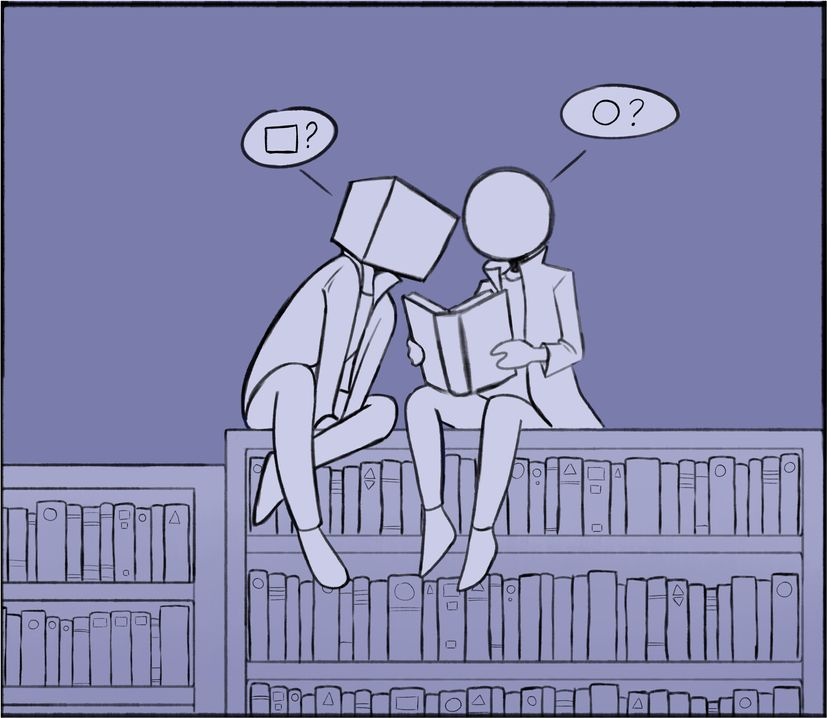
\includegraphics[width=6.5cm]{img/Illustration2-reduced.jpg}
\end{minipage}
\\
\end{tabular}

\medskip
In addition, each system has its own definitions of various
mathematical objects and structures that must be aligned: structural
results proved for one definition of real numbers, for instance, will
be transported to any isomorphic structure, regardless of the way it
has been defined. This is a final objective of this project.  Its
performance indicator is the number of proofs we are able to bring
from level LIL 4 to level LIL 5.
%%%%%%%%%%%%%%%%%%%%%%%%%%%%%%%%%%%%%%%%%%%%%%%%%%%%%%%%%%%%%%%%%%%%%%%%%%%%%%
\begin{longtable}{|p{0.2\textwidth}|p{0.4\textwidth}|p{0.32\textwidth}|}
\hline
\rowcolor{color2}
{\bf Objective}
&
{\bf Activity to achieve this objective}
&
{\bf Performance indicator}\\
\hline
{\bf Integration of proof systems}
&
Integrate the librairies of Matita, HOL Light, FoCaLiZe, Coq,
Isabelle/HOL, Agda, Atelier B, Rodin, and HOL4.
&
\vspace*{-0.41cm}

\hspace*{-0.24cm}
\begin{tabular}{p{0.127\textwidth}|p{0.07\textwidth}|p{0.07\textwidth}}
System & current & targeted\\
\hline
Matita & LIL 5 & LIL 6\\
\hline
HOL Light & LIL 3 & LIL 5\\
\hline
FoCaLiZe & LIL 3 & LIL 5\\
\hline
Coq & LIL 3 & LIL 5\\
\hline
Isabelle/HOL & LIL 2 & LIL 5\\
\hline
Agda & LIL 2 & LIL 4\\
\hline
Atelier B & LIL 1 & LIL 5\\
\hline
Rodin & LIL 1 & LIL 3\\
\hline
HOL4 & LIL 1 & LIL 5\\
\end{tabular}
\\
\hline
{\bf Integration of automated theorem proving}
&
Integrate proofs coming from automated
theorem provers and SMT solvers.
&
\vspace*{-0.41cm}

\hspace*{-0.24cm}
\begin{tabular}{p{0.127\textwidth}|p{0.07\textwidth}|p{0.07\textwidth}}
Format & current & targeted\\
\hline
TSTP & LIL 1 & LIL 4\\
\hline
LFSC & LIL 0 & LIL 4\\
\hline
Why3 & LIL 0 & LIL 4\\
\end{tabular}
\\
\hline
{\bf Integration of big libraries}
&
Integrate the Isabelle Archive of formal proofs, the Isabelle
probability and analysis library, the Coq geometry library, the
Flyspeck library, and the CakeML library.
&
\vspace*{-0.41cm}

\hspace*{-0.24cm}
\begin{tabular}{p{0.127\textwidth}|p{0.07\textwidth}|p{0.07\textwidth}}
Library & current & targeted\\
\hline
AFP & LIL 2 & LIL 4\\
\hline
Probability / analysis & LIL 2 & LIL 4\\
\hline
GeoCoq & LIL 2 & LIL 4\\
\hline
Flyspeck & LIL 2 & LIL 4\\
\hline
CakeML & LIL 2 & LIL 4\\
\end{tabular}
\\
\hline
{\bf Development of the infrastructure}
&
Make Logipedia freely accessible through a web browser and a
package distribution system. Develop a search engine for mathematical formulas.
&
TRL 4, as our target is beyond a proof of concept validated in an 
academic and industrial environment.
\\
\hline
{\bf Structuring the encyclopedia}
&
Structure the content of Logipedia into libraries, books, chapters,
etc., reaping the benefit of the structure (modules, qualified names,
etc.) of some of the libraries we start with, and enrich the data
with meta-data.
&
TRL 4, as our target is beyond a proof of concept validated in an 
academic and industrial environment.
\\
\hline
{\bf New theories, new systems}
&
Express the theories of Mizar, \tlaplus, PVS, Minlog, ProvenTools,
K Prover, and Homotopy type theory in Dedukti.
&
\vspace*{-0.41cm}

\hspace*{-0.24cm}
\begin{tabular}{p{0.127\textwidth}|p{0.07\textwidth}|p{0.07\textwidth}}
System & current & targeted \\
\hline
Mizar & LIL 0 & LIL 4\\
\hline
\tlaplus & LIL 0 & LIL 2\\
\hline
PVS & LIL 0 & LIL 2\\
\hline
Minlog & LIL 0 & LIL 4\\
\hline
ProvenTools & LIL 0 & LIL 3\\
\hline
K Prover & LIL 0 & LIL 3\\
\hline
Homotopy type theory & LIL 0 & LIL 3\\
\end{tabular}
\\
\hline
{\bf Proof engineering}
&
Develop algorithms to analyze which axioms are used in a proof,
eliminate them, and align concepts.
&
Bringing 25\% of the encyclopedia to LIL 5, that is making
the proofs of a significant part of the library available in systems
different from those in which they have been developed.
\\ \hline
\end{longtable}

The seven objectives give a first idea of the shape of the project.

They all contribute to building a new formal proof community, focused
on the values of knowledge sharing, safety, security, privacy, open
access, and education.

%%% Local Variables:
%%%   mode: latex
%%%   mode: flyspell
%%%   ispell-local-dictionary: "english"
%%% End:
